\documentclass{article}
\usepackage{packages}

\begin{document}
\centerline{\Large\bfseries Matteo Zortea}
\vspace{10pt}
\centerline{\Large\bfseries Fundamentals of Simulation Methods}
\vspace{10pt}
\centerline{\Large\bfseries Sheet 12}
\vspace{30pt}

\subsubsection*{(a)}
See 1p.mp4.

\subsubsection*{(b)}
Since we are in hydrostatic equilibrium we expect the local flow speed to be zero, on average.

\subsubsection*{(c)}
A lower softening length would result in more particle scattered (allowance for higher accelerations) but also in a higher 
probability of numerical problems. \\
A higher softening length would contain numerical errors, but also alterate the physics, preventing particles to be accelerated as they should be. \\
I expect that the higher the softening length, the higher the deviation from energy conservation.

\subsubsection*{(d)}
The Mach number indicates the ratio of the local flow velocity and the speed of sound. 
If the local flow speed is negligible with respect to the sound speed, we can consider the planet at rest in the medium (hydrostatic equilibrium). \\
In particular one can consider the time required to shift the planet by its own radius. Due to pure speed sound velocity this time would be $t_1 = \frac{R}{\left\langle C_s \right\rangle}$, while for pure 
flow velocity it would be $t_2 = \frac{R}{\left\langle |\mathbf{v}| \right\rangle}$. The ratio of the two times is exactly the Mach number  
\begin{equation*}
    \left\langle M \right\rangle = \frac{\left\langle |v| \right\rangle}{\left\langle C_s \right\rangle}
\end{equation*}
\begin{figure}[h]
    \centering 
    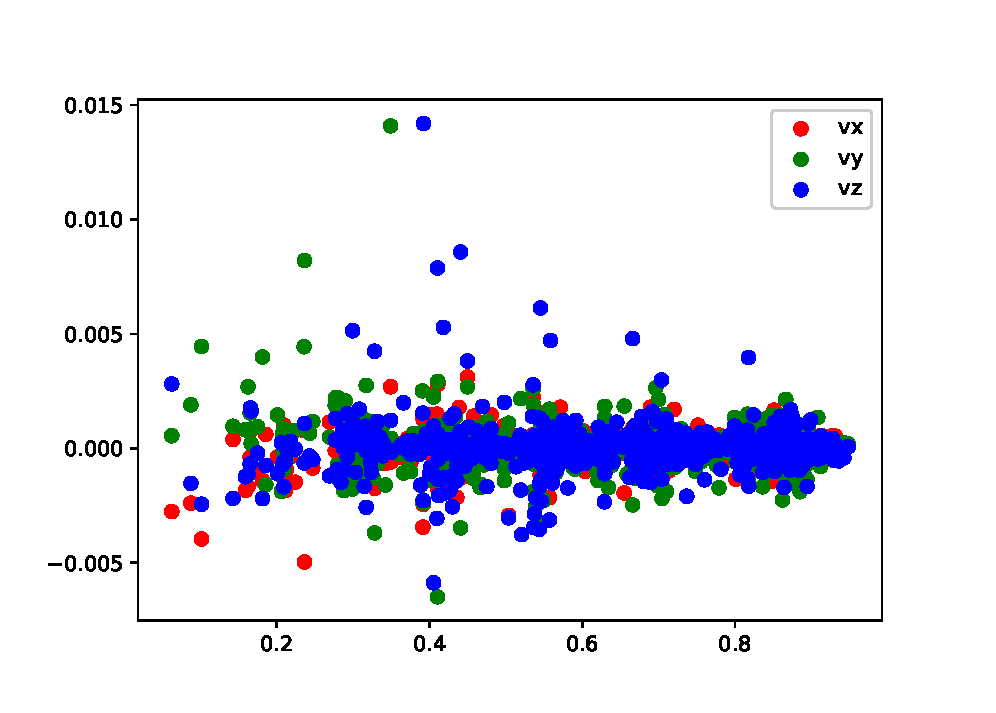
\includegraphics[scale=0.9]{mach.eps}
    \caption{Mach number}
    \label{fig:mach}
\end{figure}
Which is plotted in figure \ref{fig:mach} for each particle.

\subsubsection*{(e)}
See 2p.mp4.

\subsubsection*{(f)}
The plots are reported in figure \ref{fig:energy}.
\begin{figure}[h]
    \centering
    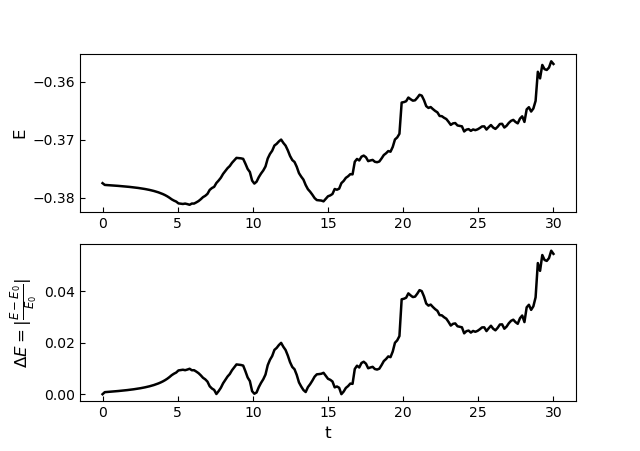
\includegraphics[scale=0.9]{energy.png}
    \caption{Energy conservation}
    \label{fig:energy}
\end{figure}

\end{document}